\documentclass[10pt,a4paper]{article}
\usepackage[latin1]{inputenc}
\usepackage{amsmath}
\usepackage{amsfonts}
\usepackage{amssymb}
\usepackage{pdfpages}
\usepackage{rotating}
\begin{document}
\begin{center}
\Huge{Project plan}\\[.2cm]
\Large{A Graphical User Interface (GUI) for weather radar and wind energy data visualization and analysis}\\[.2cm]
February 2012
\end{center}
Mads Lundt, s103439\\
Matthias, s103437\\
Joachim Jensen, s103430

\section{Analysis}
From the project description on CampusNet:

"\emph{Background: Wind energy applications such as wind power prediction require the use of large amounts of data. These data come from multiple sources (e.g. onsite observations from measuring stations, meteorological forecasts from Numerical Weather Prediction models, images from weather radars) and, consequently, have very diverse formats (times series, georeferenced data, gridded data). This raises an important issue since there does not exist any common or efficient platform for their visualization and analysis.}

\emph{The objective is to design a user-friendly GUI for enhancing the combined visualization of several sources of data. The following initial specifications will serve as a starting point for the project: }
\begin{itemize}
\item \emph{efficient system for data request, retrieval and display}
\item \emph{handling of animations (it is crucial as most data consist of  time series or of series of images)}
\item \emph{preferences should be given to open source softwares/programming languages/solutions}
\item \emph{operationability of the final GUI on web browsers will be considered}
\end{itemize} 
"

\section{Solution strategy}
Based on the analysis of the project, our solution will be solely webbased using an interactive map with several data layers shown in an intuitive way.

We have discussed the use of the following technologies: PHP, JavaScript, HTML5, CSS3, C/C++, XML.\\
And the following frameworks: Node.js, jQuery, FuelPHP, Qt.

As visualising of the data we have chosen to make use of a map like Google Maps and OpenStreetMap. The most important thing is that it's open source. 

\section{Estimated resources}
1 cola per working hour and a large amount of electricity.

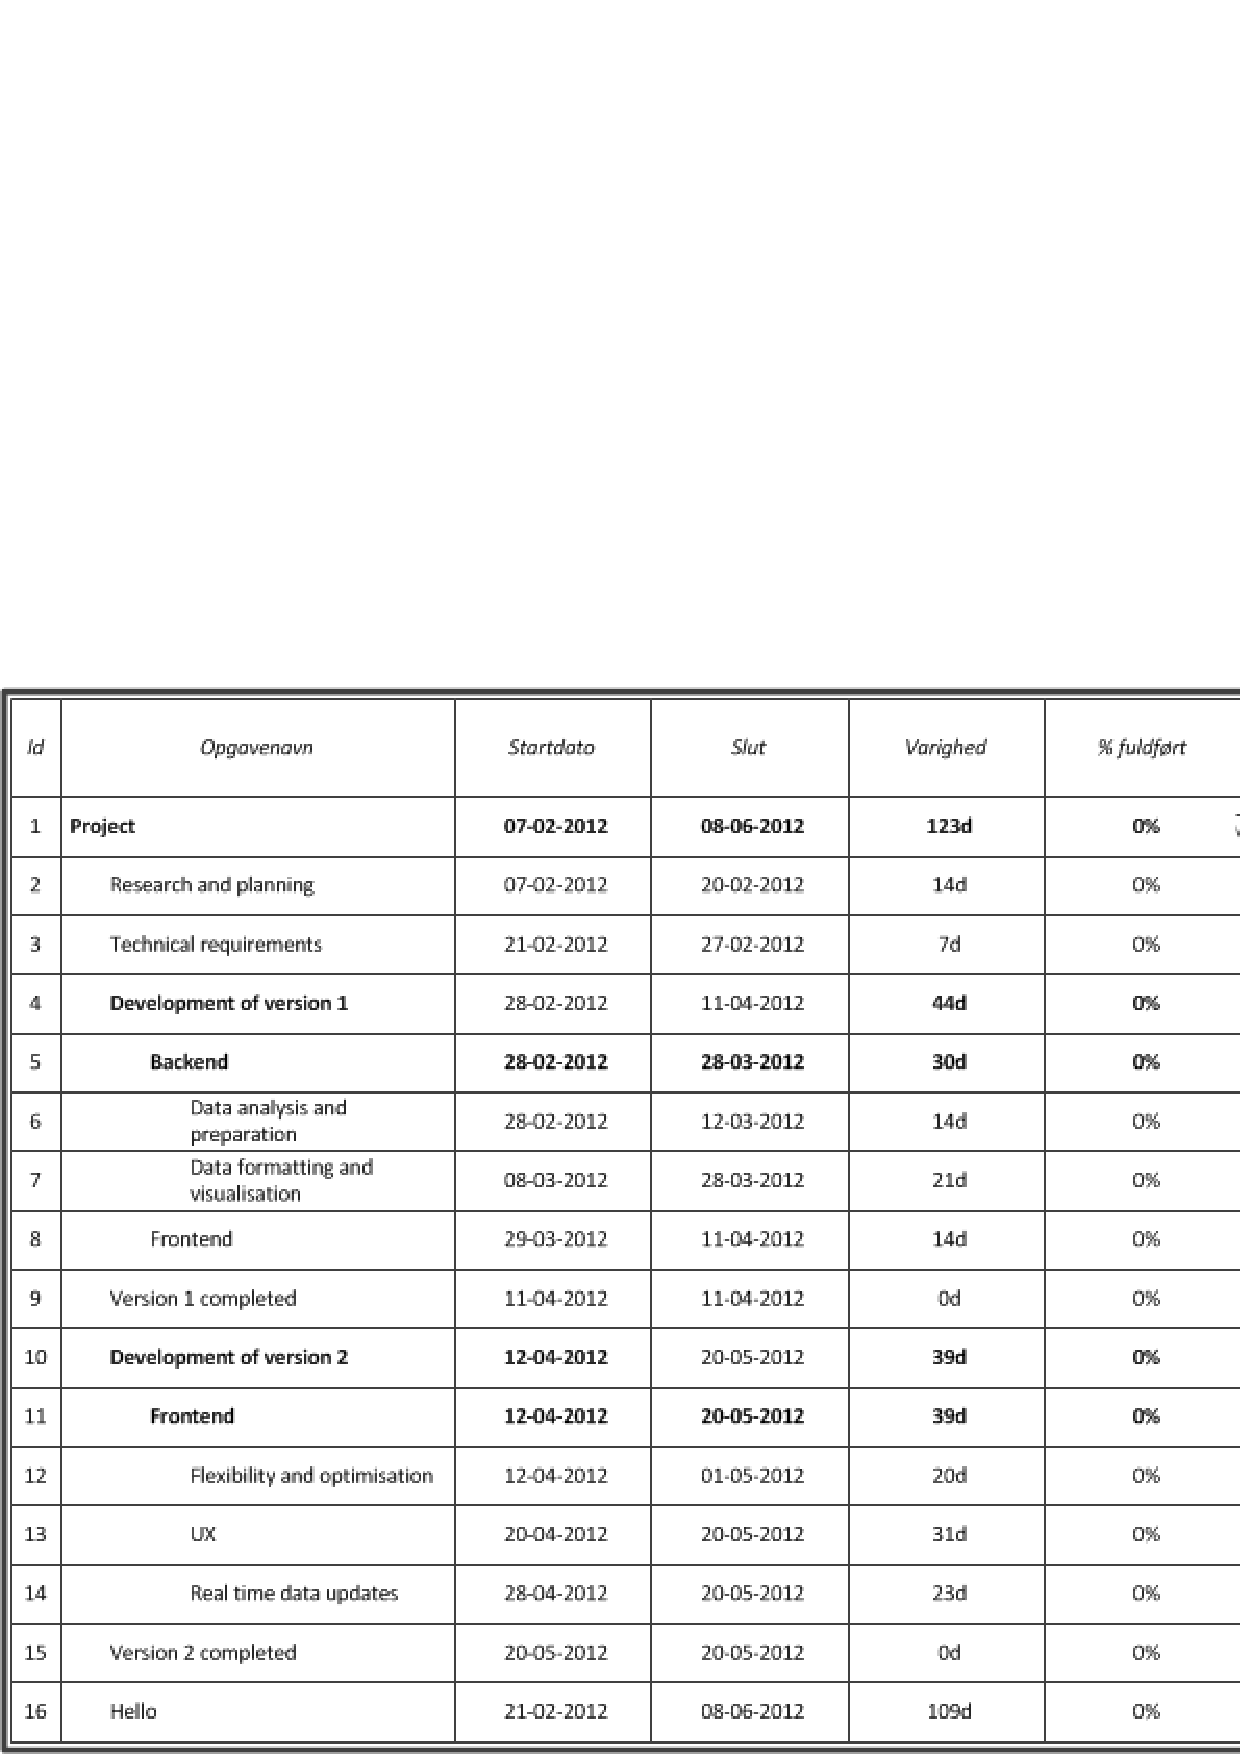
\includepdf[scale=0.7,pagecommand=\section{Time schedule}]{planning1}

\section{Work destribution}
To be decided after meeting with supervisors.

\end{document}